\pagebreak
\section{Automatic Generation Control}  \label{sec: AGC def}
Automatic generation control (AGC) is an extended-term model that acts to restore system frequency and area interchange values to set values over the course of minutes.
This restoration is accomplished by calculating an area control error (ACE) that is distributed to controlled generation sources to correct any deviation from reference values.

%model calculates an area control error (ACE) and distributes it to defined controlled generators according to participation factor.
%The ACE signal is passed through a PI filter before being distributed to each generator through a unique low pass filter that adds the negative of the value to the governor \verb|tg_sig| value.
%( NOTE: the \verb|tg_sig| value is equivalent to an addition to the governors $P_{ref}$ value)
%The \verb|agc_indx| function creates the required data structures and indices.

%==========================================================================
\subsection{AGC Block Diagrams}
The AGC process is shown in Figures \ref{fig: agc block diagram 1}, \ref{fig: agc block diagram 2}, and \ref{fig: agc block diagram 3}.
$RACE$ (reporting ACE) and SACE (smoothed ACE) are calculated using PU values assuming $B$ is a positive non-PU value with units of $MW/0.1Hz$.
If $K_{bv}$ is not zero, the resulting $RACE$ is not the industry standard (WECC defined) $RACE$ value.
The scheduled interchange may be altered by the user via a \verb|mAGC_sig| file that controls the behavior of the $IC_{adj}$ input.

% NOTE: say something about an example?

\begin{figure}[!h]
	\centering
	\footnotesize
	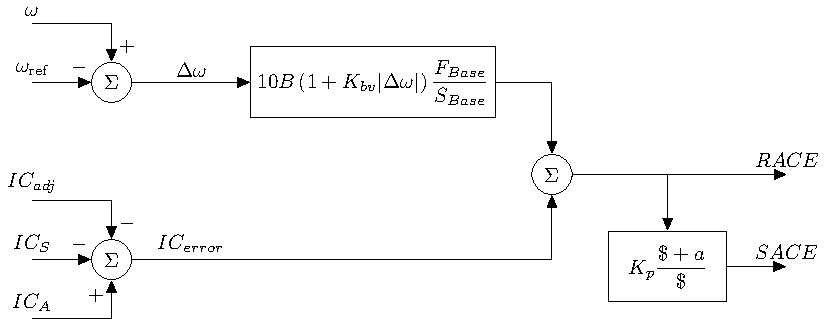
\includegraphics[width=\linewidth]{sections/agc/200722-AGCblockdiagram-p1}
	\caption{AGC calculation of $RACE$ and $SACE$.}
	\label{fig: agc block diagram 1}
\end{figure}%\vspace{-1 em}

\pagebreak
$RACE$ and $SACE$ are calculated every simulation time step, however
distribution of $SACE$ is determined by the user defined \verb|startTime| and \verb|actionTime| variables.
Assuming action, the conditional $\Delta\omega$ logic is processed before adjusting the \verb|aceSig| value which is then gained to become \verb|ace2dist|.

\begin{figure}[!h]
	\centering
	\footnotesize
	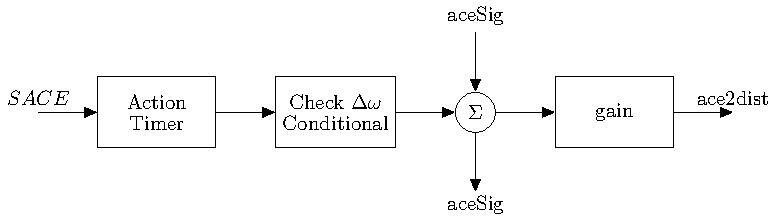
\includegraphics[width=\linewidth]{sections/agc/200722-AGCblockdiagram-p2}
	\caption{AGC calculation of $ace2dist$.}
	\label{fig: agc block diagram 2}
\end{figure}%\vspace{-1 em}

The \verb|ace2dist| value is distributed to all controlled generators associated with the AGC model according to their respective participation factor \verb|pF|.
Each \verb|ctrlGen| has a unique low pass filter to allow for different `ramping' of signals to individual machines.
The output of the low pass filter is gained by -1 and added to the existing associated governor \verb|tg_sig| value to drive ACE to zero.

\begin{figure}[!h]
	\centering
	\footnotesize
	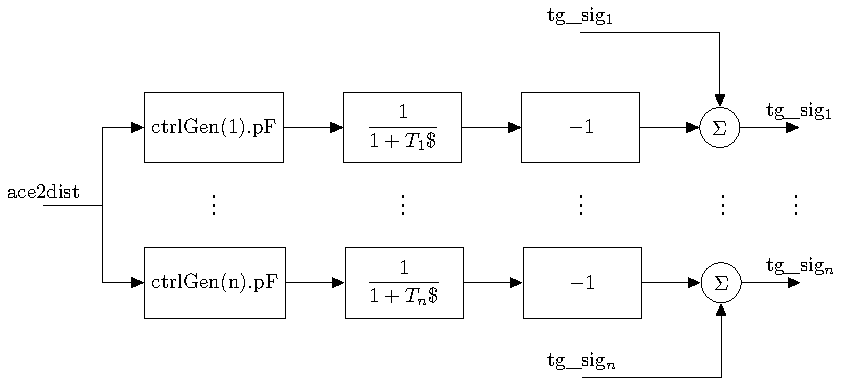
\includegraphics[width=\linewidth]{sections/agc/200722-AGCblockdiagram-p3}
	\caption{AGC handling of $ace2dist$ to individual governor signals.}
	\label{fig: agc block diagram 3}
\end{figure}%\vspace{-1 em}




%==================================================
\pagebreak
\subsection{AGC Definition Example}
The following AGC settings are not realistic, but useful in demonstrating the required user definitions and functionality of the AGC model.
Settings from one AGC model can be easily copied to another using \verb|agc(2) = agc(1)| and then changing the area number and \verb|ctrlGen_con| array as desired.

\begin{minted}[
		frame=lines,
		framesep=2mm,
		baselinestretch=1.2,
		bgcolor=gray!13,
		fontsize=\footnotesize,
		%linenos,
		breaklines
		]{MATLAB}
%{  
AGC definition. Each agc(x) has following fields:
    area        - Area Number 
    startTime   - Time of first AGC signal to send
    actionTime  - Interval of time between all following AGC signals
    gain        - Gain of output AGC signal
    Btype       - Fixed frequency bias type
        0 - absolute - Input B value is set as Frequency bias (positive MW/0.1Hz)
        1 - percent of max area capacity
    B           - Fixed frequency bias value
    Kbv         - Varaible frequency bias gain used to gain B as B(1+kBv*abs(delta_w))
    condAce     - Conditional ACE flag
        0 - Conditional ACE not considered
        1 - ace2dist updated only if sign matches delta_w (i.e. in area event)
    Kp          - Proportional gain
    a           - ratio between integral and proportional gain (placement of zero)
    ctrlGen_con - Controlled generator information
        column 1 - Generator External Bus Number
        column 2 - Participation Factor
        column 3 - Low pass filter time constant [seconds]
%}
agc(1).area = 1;
agc(1).startTime = 25;  % seconds
agc(1).actionTime = 15; % seconds
agc(1).gain = 2;        % gain of output signal
agc(1).Btype = 1;       % per max area capacity
agc(1).B = 1;           % Use 1% of max area capacity as B
agc(1).Kbv = 0;         % no variable bias
agc(1).condAce = 0;     % conditional ACE ignored
agc(1).Kp = 0.04;       % PI proportional gain
agc(1).a = 0.001;       % Ratio between integral and proportional gain
agc(1).ctrlGen_con = [ ...
    1, 0.75, 15;
    2, 0.25, 2;  ];
\end{minted}



%==========================================================================

\subsection{Weighted Average Frequency (calcAveF)} 
An inertia weighted average frequency is used as the `actual' frequency $\omega$ in ACE calculations.
The \verb|calcAveF| function calculates an average weighted frequency for the total system and for each area (if areas are defined).
System values are stored in \verb|g.sys.aveF| and area values are stored in \verb|g.area.area(x).aveF| where \verb|x| is the internal area number.
The calculation involves a sum of system inertias that changes with generator trips.


\vspace{1em}
In a system with $N$ generators, $M$ areas, and $N_M$ generators in area $M$, the \verb|calcAveF| function performs the following calculations for each area $M$:

\begin{equation}{\label{eq: areaH} }
H_{tot_M} = \sum_{i}^{N_M} MVA_{base_i}H_i
\end{equation}\eqcaption{Area Inertia Calculation} 
\vspace{-1em}
\begin{equation}{\label{eq: areaF} }
F_{ave_M} = \left( \sum_{i}^{N_M}Mach_{speed_i}MVA_{base_i}H_i \right) \dfrac{1}{H_{tot_M}}
\end{equation}\eqcaption{Area Average System Frequency Calculation}
\vspace{0.5 em}

\noindent System total values are calculated as:

\begin{equation}{\label{eq: systemH} }
H_{tot} = \sum_{i}^{M} H_{tot_M}
\end{equation}\eqcaption{System Inertia Calculation} 
\vspace{-1em}
\begin{equation}{\label{eq: systemF} }
F_{ave} = \left( \sum_{i}^{M} F_{ave_M} \right) \dfrac{1}{M}
\end{equation}\eqcaption{System Average System Frequency Calculation}
\vspace{0.5 em}

\noindent If $M==0$ (areas are not defined), \verb|calcAveF| performs:

\begin{equation}{\label{eq: systemH2} }
H_{tot} = \sum_{i}^{N} MVA_{base_i}H_i 
\end{equation}\eqcaption{Area-less System Inertia Calculation} 
\vspace{-1em}
\begin{equation}{\label{eq: systemF2} }
F_{ave} = \left( \sum_{i}^{N}Mach_{speed_i}MVA_{base_i}H_i \right) \dfrac{1}{H_{tot}}
\end{equation}\eqcaption{Area-less System Average System Frequency Calculation}\vspace{0.5 em}

\pagebreak
%==================================================
\subsection{Other Area Calculations (calcAreaVals)}  
The \verb|calcAreaVals| function calculates real and reative power generated by all area machines and actual area interchange every time step.
It should be noted that power injected via loads, pwrmod, or ivmmod are not included in the \verb|g.area.area(n).totGen(k)| value.
An area's actual interchange is calculated using the \verb|line_pq2| function to collect area to area line power flows.
